\documentclass{article}

\usepackage{array}
\usepackage{tabularx}

\usepackage{amssymb}

\usepackage{comment}

\usepackage{tcolorbox}

\usepackage{graphicx}
\usepackage{subcaption}

\usepackage{amsmath}

\usepackage{float}

\usepackage[export]{adjustbox}

\usepackage[margin=1.25in]{geometry}

\newtcbox{\inlinecode}{on line, boxrule=0pt, boxsep=0pt, top=2pt, left=2pt, bottom=2pt, right=2pt, colback=gray!15, colframe=white, fontupper={\ttfamily \footnotesize}}

\begin{document}

\begin{center}
        \textbf{Robotics/Engineering 101}
        
        \vspace*{12pt}

        \textbf{Electronic Circuits Week} \\
        7/28/2022 \\
        \vspace*{12pt}
        Worksheet by Dylan Kirdahy 
\end{center}

\pagenumbering{arabic}

Check the boxes when you've completed an activity, or fill in the blanks with answers/measurements.

\section{Simple Circuits}

\paragraph{}
In this section, you will build some very simple circuits in order to learn the basics of using a breadboard and wires.

\subsection{Buzzer Circuit}
\paragraph{}
Wire up the active buzzer to the power rails of the breadboard.
\begin{figure}[H]
  \centering
  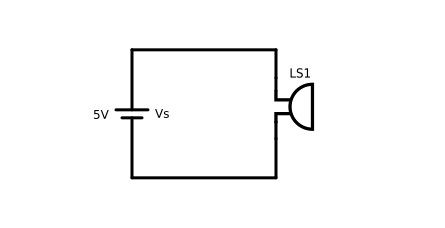
\includegraphics[width=0.4\linewidth]{pngs/01-buzzer.png}
\end{figure}
\paragraph{}
$\square$ Circuit built, and buzzer makes sound

\subsection{Motor Circuit}
\paragraph{}
Now wire up a motor to the power rails instead.
\begin{figure}[H]
  \centering
  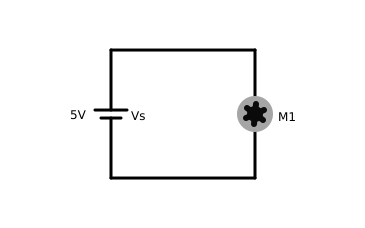
\includegraphics[width=0.4\linewidth]{pngs/02-dc-motor.png}
\end{figure}
\paragraph{}
$\square$ Circuit built, and motor spins

\pagebreak
\subsection{LED Circuit}
\paragraph{}
Wire an LED to the power rails, placing a resistor in series with it. The resistor is called a "current limiting resistor" in this scenario, and it makes sure the LED does not draw too much current and break. Make sure the polarity of the LED is correct: the shorter lead goes to ground (0V) and the longer lead goes to 5V.
\begin{figure}[H]
  \centering
  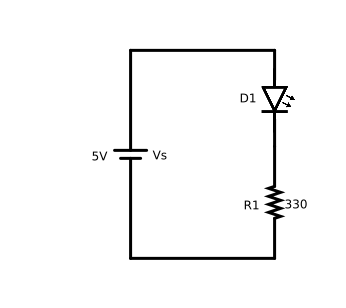
\includegraphics[width=0.4\linewidth]{pngs/03-led.png}
\end{figure}
\paragraph{}
$\square$ Circuit built, and LED lights up

\subsection{LED Circuit With Button}
\paragraph{}
Now place a button in series with the LED. The button goes into the middle of the breadboard. The leads with the same curve go on the same side of the breadboard, as shown in the image. The two leads on the same side of the breadboard are the leads you connect to when wiring. If the button conducts even when it's not pressed, you need to turn it 90 degrees.
\begin{figure}[H]
  \centering
  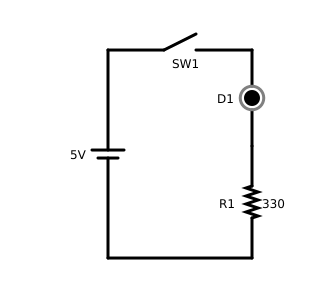
\includegraphics[width=0.4\linewidth]{pngs/04-led-button.png}
  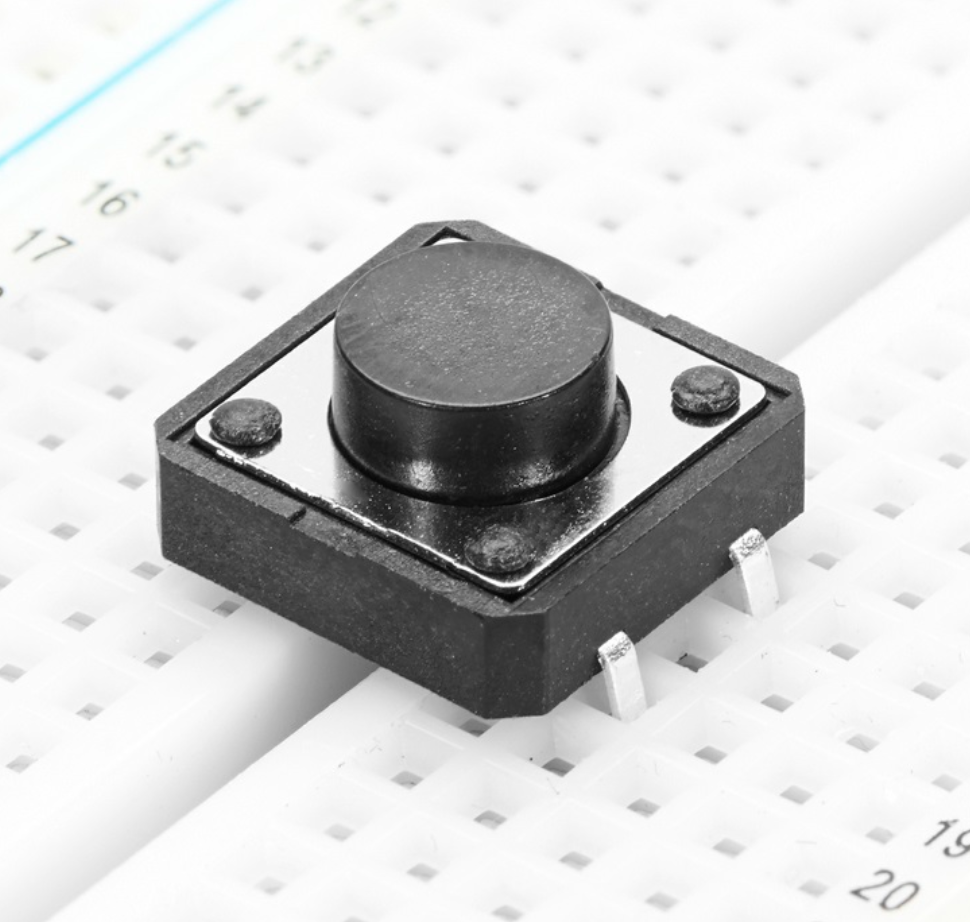
\includegraphics[width=0.4\linewidth]{pngs/button.png}
\end{figure}
\paragraph{}
$\square$ Circuit built, and LED lights up only when button is pushed03-led.png

\newpage
\subsection{LED Circuit With Different Resistances}
\paragraph{}
Now try different resistance values with the LED. When you try higher values, the LED should be dimmer, and lower values should make it brighter. Write down the values you tried. Feel free to try different colors of LEDs too!
\begin{figure}[H]
  \centering
  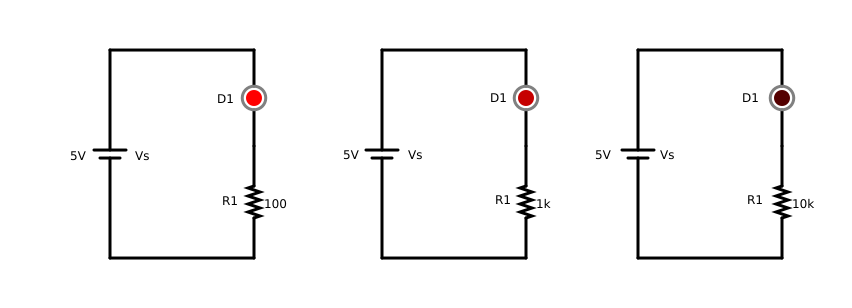
\includegraphics[width=0.6\linewidth]{pngs/05-led-multiple-resistances.png}
\end{figure}
\noindent
Resistor value 1: \rule{4cm}{0.15mm} Brightness observed: \rule{4cm}{0.15mm}
\newline
\newline
Resistor value 2: \rule{4cm}{0.15mm} Brightness observed: \rule{4cm}{0.15mm}
\newline
\newline
Resistor value 3: \rule{4cm}{0.15mm} Brightness observed: \rule{4cm}{0.15mm}

\newpage
\section{Basic Circuit Theory}
Now you will learn some basic circuit theory! You'll be doing some simple calculations about demo circuits, and then you'll build the circuits yourselves and take measurements. You can compare your calculations and measurements to confirm the circuit theory equations.

\subsection{Ohm's Law}
\paragraph{}
Now you're going to confirm that Ohm's Law (V=IR) is true. Ohm's law says that the voltage across a resistor is proportional to the resistance and the current flowing through the resistor. Try different resistor values and see what happens to the current!
\begin{figure}[H]
  \centering
  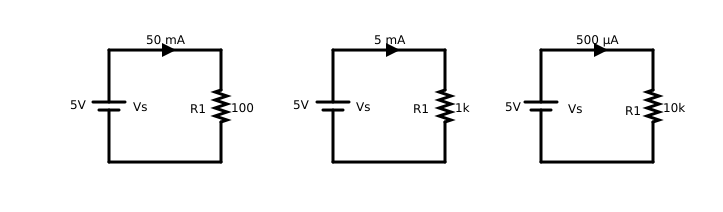
\includegraphics[width=0.8\linewidth]{pngs/06-resistor-current-measurement.png}
\end{figure}
\paragraph{}
Plug the battery voltage and resistor values of your choosing into Ohm's Law (as shown below) to calculate the current. Then, build the circuit and measure the current to confirm your calculations.
\begin{equation*}
  I = \frac{V}{R}
\end{equation*}
\noindent
Resistor value 1: \rule{2cm}{0.15mm} Expected current: \rule{2cm}{0.15mm} Measured current: \rule{2cm}{0.15mm}
\newline
\newline
Resistor value 2: \rule{2cm}{0.15mm} Expected current: \rule{2cm}{0.15mm} Measured current: \rule{2cm}{0.15mm}
\newline
\newline
Resistor value 3: \rule{2cm}{0.15mm} Expected current: \rule{2cm}{0.15mm} Measured current: \rule{2cm}{0.15mm}
\newline
\newline

\newpage
\subsection{Resistors in Series}
\subsubsection{Total Resistance}
\paragraph{}
Resistance values add up in series. In the following circuit, the total resistance is calculated like so:
\begin{equation*}
  R_{total} = R_1 + R_2
\end{equation*}
\paragraph{}
\begin{figure}[H]
  \centering
  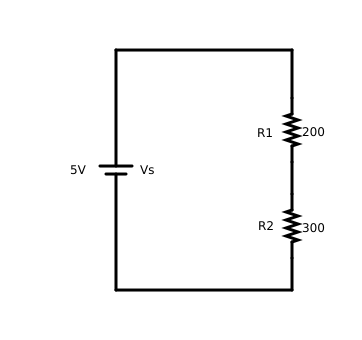
\includegraphics[width=0.4\linewidth]{pngs/07-resistors-series.png}
\end{figure}
\paragraph{}
The total resistance is 500 ohms in this case.

\subsubsection{Current}
The current through the circuit is calculated as follows.
\begin{equation*}
  I = \frac{V}{R_1+R_2}
\end{equation*}
 Notice how the current going through both resistors is the same!
\begin{figure}[H]
  \centering
  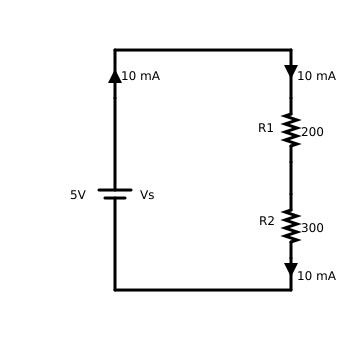
\includegraphics[width=0.4\linewidth]{pngs/07-resistors-series-current.png}
\end{figure}

\subsubsection{Voltage}
\paragraph{}
The voltage across a resistor is dictated by V=IR, so we can plug in the current formula from above to get the voltage drop on R1, for instance:
\begin{equation*}
  V_{R1} = \frac{V}{R_1+R_2}*R_1
\end{equation*}
\paragraph{}
Notice how the voltage across the resistors are different! Also notice how the voltages add up to the voltage of the power supply.
\begin{figure}[H]
  \centering
  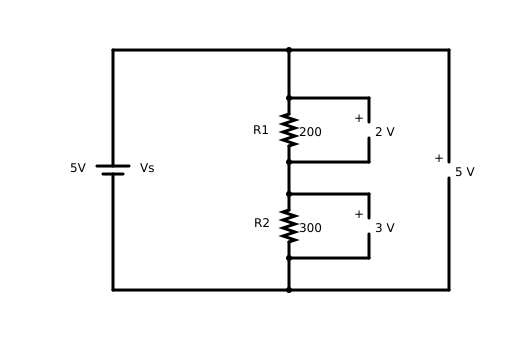
\includegraphics[width=0.6\linewidth]{pngs/07-resistors-series-voltage.png}
\end{figure}
\paragraph{}
(Note that the resistor values in the above schematics are for example purposes. Choose your own values in the activity!)

\subsubsection{Activity}
\noindent
Choose two resistor values from your kit. R$_1$ value: \rule{2cm}{0.15mm} R$_2$ value: \rule{2cm}{0.15mm}
\newline
\newline
Calculate the total resistance. R$_{total}$ = \rule{2cm}{0.15mm} 
\newline
\newline
Calculate the current flowing through the circuit. I = \rule{2cm}{0.15mm} 
\newline
\newline
Calculate the voltage across R$_1$. V$_{R1}$ = \rule{2cm}{0.15mm} 
\newline
\newline
Calculate the voltage across R$_2$. V$_{R2}$ = \rule{2cm}{0.15mm} 
\newline
\newline
\newline
\newline
Now build the circuit and make measurements to check your calculations!
\newline
\newline
Measure the total resistance. (You will have to disconnect power to measure properly) 
\newline
\newline
Rtotal = \rule{2cm}{0.15mm} 
\newline
\newline
Measure the current through the circuit. I = \rule{2cm}{0.15mm} 
\newline
\newline
Measure the voltage drops. V$_{R1}$ = \rule{2cm}{0.15mm} V$_{R2}$ = \rule{2cm}{0.15mm} 












\end{document}
